\chapter{Theory}

This chapter outlines the current theory for neutrinos and that of double beta decay.  Theory relevant to the spectroscopy of Ba in SXe is then discussed.

\emph{{\color{gray}See more Leif examples of some things.}}

\section{Neutrinos}

Neutrinos are chargeless leptons which only interact via the weak force (and gravity).  There are three known ``flavors'' of neutrinos, each corresponding to one of the three known leptons:  $\nu_{e}$, $\nu_{\mu}$, and $\nu_{\tau}$.  These are the eigenstates in the basis of the weak force, and so they are the states in which a neutrino will interact via the weak force.

{\color{gray}\emph{History:  }Neutrinos were first proposed while studying beta decay.  If the emitted electron and daughter nucleus in beta decay were the only products, the electron's energy should be essentially the same for every observed beta decay for a given isotope, since there is a certain energy difference between the initial and final states of the nucleus, and since the final kinetic energy of the nucleus is negligible due to its mass.  But instead of a sharp peak at this Q-value, a very broad electron energy spectrum is observed, all beneath and decreasing toward the Q-value.

In 1930, Wolfgang Pauli proposed that this variable ``loss'' in energy could be due to an additional particle being emitted along with the electron, but which is not observed.

[Fermi, massless]

[observation, and discovery of nu mu]}

\subsection{Neutrino Oscillation and Mass}

Neutrinos exhibit mixing between their energy eigenstates and their weak force eigenstates, and these are not the same basis.  This means that a flavor eigenstate is not a stationary state --- a neutrino which begins as a pure flavor state (as all neutrinos will, coming out of a quantum process involving one of the three leptons) will oscillate into the other two flavors as it evolves in time, i.e. the probability of measuring it to be one of the other two flavors is no longer zero.

{\color{gray}\emph{History:  }The first indications of neutrino oscillation came around 1970 with the Ray Davis Experiment [ref.], which measured the flux (at Earth) of solar electron neutrinos.  The flux measured was quite a bit lower than predicted by solar models, and this became known as the Solar Neutrino Problem.  The discovery of neutrino oscillation in the late 1990s [ref.] solved this problem, as only a fraction of the sun's neutrinos, produced as pure electron neutrinos, would interact as such.}

The very small mass of a neutrino, specifically relative to its momentum, lets one write its Hamiltonian in terms of mass squared differences $\Delta m_{ij}^{2} = m_{i}^{2} - m_{j}^{2}$, where $i$,$j$ = 1,2,3, referring to what we then call mass states.  The mass basis is really the energy basis with the small mass approximation, along with dropping some constant terms in the Hamiltonian (which do not affect time evolution).  Writing the time evolution in terms of mass squared differences means that neutrino oscillation experiments can produce measurements of these differences.  In fact, the discovery of neutrino oscillation was the first (and only, so far) demonstration that neutrinos have a non-zero mass.  Without neutrino mass (particularly without differences between the masses of the mass states), neutrinos would not oscillate.

Neutrino oscillation experiments also provide measurements on the amount of mixing between the flavor basis and the mass basis.  We define the mixing between them by a rotation in terms of three mixing angles, $\theta_{12}$, $\theta_{23}$, and $\theta_{13}$.  Transformation between the flavor and mass bases is done with the following unitary matrix, called the Pontecorvo--Maki-–Nakagawa–-Sakata (PMNS) matrix:

\begin{equation}
\begin{aligned}
U &= \begin{pmatrix}
1 & 0 & 0 \\
0 & c_{23} & s_{23} \\
0 & -s_{23} & c_{23} \end{pmatrix}
\begin{pmatrix}
c_{13} & 0 & s_{13} e^{-i \delta} \\
0 & 1 & 0 \\
-s_{13} e^{i \delta} & 0 & c_{13} \end{pmatrix}
\begin{pmatrix}
c_{12} & s_{12} & 0 \\
-s_{12} & c_{12} & 0 \\
0 & 0 & 1 \end{pmatrix}
\begin{pmatrix}
1 & 0 & 0 \\
0 & e^{i \alpha_{1}/2} & 0 \\
0 & 0 & e^{i \alpha_{2}/2} \end{pmatrix} \\
& = \begin{pmatrix}
c_{12} c_{13} & s_{12} c_{13} & s_{13} e^{-i \delta} \\
-s_{12} c_{23} - c_{12} s_{23} s_{13} e^{i \delta} & c_{12} c_{23} - s_{12} s_{23} s_{13} e^{i \delta} & s_{23} c_{13} \\
s_{12} s_{23} - c_{12} c_{23} s_{13} e^{i \delta} & -c_{12} s_{23} - s_{12} c_{23} s_{13} e^{i \delta} & c_{23} c_{13} \end{pmatrix}
\begin{pmatrix}
1 & 0 & 0 \\
0 & e^{i \alpha_{1}/2} & 0 \\
0 & 0 & e^{i \alpha_{2}/2} \end{pmatrix}
\end{aligned}
\label{eqn:umatrix}
\end{equation}

\noindent
where $c_{ij} = \cos \theta_{ij}$ and $s_{ij} = \sin \theta_{ij}$.  $\delta$ is a phase factor related to lepton CP violation, and $\alpha_{i}$ are Majorana phases.

Studying oscillations of neutrinos from different kinds of sources, with different energies and path lengths, can isolate sensitivities to the different parameters {\color{gray}(not really sure if this is the right thing to say)}.  For example, the study of solar neutrinos (neutrinos emanating from nuclear fusion reactions in the core of the sun) provides sensitivity to $\theta_{12}$ and $\Delta m_{12}^{2}$ {\color{gray}(\emph{right? $\theta_{12}$ may not be specifically solar...})}.  The parameters so far measured are as follows in Table  \ref{table:nu_osc_vals}:

\begin{table}[!htbp]
\caption{up to date values with references, and denote "solar", "atmos.", etc.} %not sure what [Small Table], between \caption and {}, w/ no spaces, does
\label{table:nu_osc_vals}
\begin{tabular}{c|c}
Parameter & Measurement \\
\hline
$\Delta m_{12}^{2}$ & \\
$|\Delta m_{31}^{2}|$ & \\
$\sin^{2} \theta_{12}$ & \\
$\sin^{2} \theta_{23}$ & \\
$\sin^{2} \theta_{13}$ & \\
\end{tabular}
\end{table}

Note that only the absolute value of $\Delta m_{31}^{2}$ is known.  As a consequence, there are still two possibilities for the hierarchy of the three neutrino masses.  These are called the Normal and Inverted Hierarchies, as shown in Fig. \ref{fig:numasshier}.

\begin{figure}[H]
        \centering
                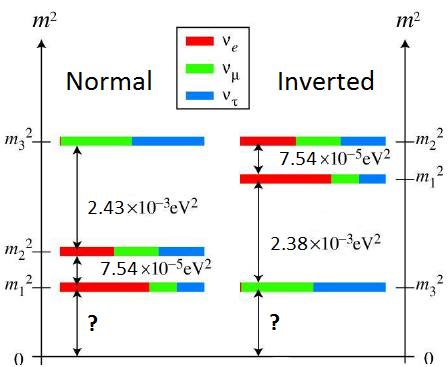
\includegraphics[width=.5\textwidth]{figures/hierarchy_alterred.png}
                \caption{The two possible hierarchies of neutrino masses.  The colors depict the mixing between the mass and flavor bases. {\color{red}\textbf{[ref]}}}
\label{fig:numasshier}
\end{figure}

Neutrino oscillation demonstrates that neutrinos have non-zero mass, and though these experiments can measure the mass squared differences, we still do not have a measurement of the absolute masses of the three neutrinos.  {\color{gray}\emph{History:  }mention Pauli's first statement of limit near electron mass?  Then maybe say the 0 assumption, which I think came from Fermi's beta decay theory, but if you mention that above, just refer to it here.}

The current upper limits on the mass come from...
Neutrinoless double beta decay experiments like EXO-200 can put upper limits on specifically the Majorana neutrino mass (i.e., upper limits on the neutrino mass if neutrinos are indeed Majorana particles).  As discussed in the next chapter, [EXO-200 and KamLAND (sp?) ZEN (sp?) together provide the strongest Majorana neutrino mass upper limit of [] (IS THAT TRUE?)].

Neutrino oscillation and non-zero neutrino mass are physics beyond the Standard Model (SM) of particle physics, and though much has been discovered through oscillation experiments, there is much yet to learn about and from neutrinos. [Majorana nature, see-saw, ... lead into next section]

\subsection{Neutrinoless Double Beta Decay}

The discovery of non-zero neutrino mass has another implication ...

\section{Barium Spectroscopy}

Do we want this here?  It flows more to have this theory after the proposition of the tagging technique, but maybe that's more appropriate for a talk.

\section{Matrix Isolation Spectroscopy}

(same thing)

